
\slidesectionwithgraphic{Conclusions}{images/stacking.png}

\begin{frame}{Conclusions}
	\begin{columns}[T,onlytextwidth]
		\begin{column}{0.5\textwidth}
			\textbf{Conclusions}
			\begin{itemize}
				\item We propose a taxonomy of treemap visualization techniques using four distinctive classes:
				\begin{description}[\Tmt]
					\item[\Ts] Space-filling Treemap 
					\item[\Tc] Containment Treemap
					\item[\Tie] Implicit-Edge Representation Tree
					\item[\Tmt] Mapped Tree
				\end{description}
				\item List of properties for each class and the term treemap in general
				\item Exemplary assignment of existing treemap and general tree visualization techniques
			\end{itemize}
		\end{column}
		\begin{column}{0.5\textwidth}
			\begin{figure}
				\centering
				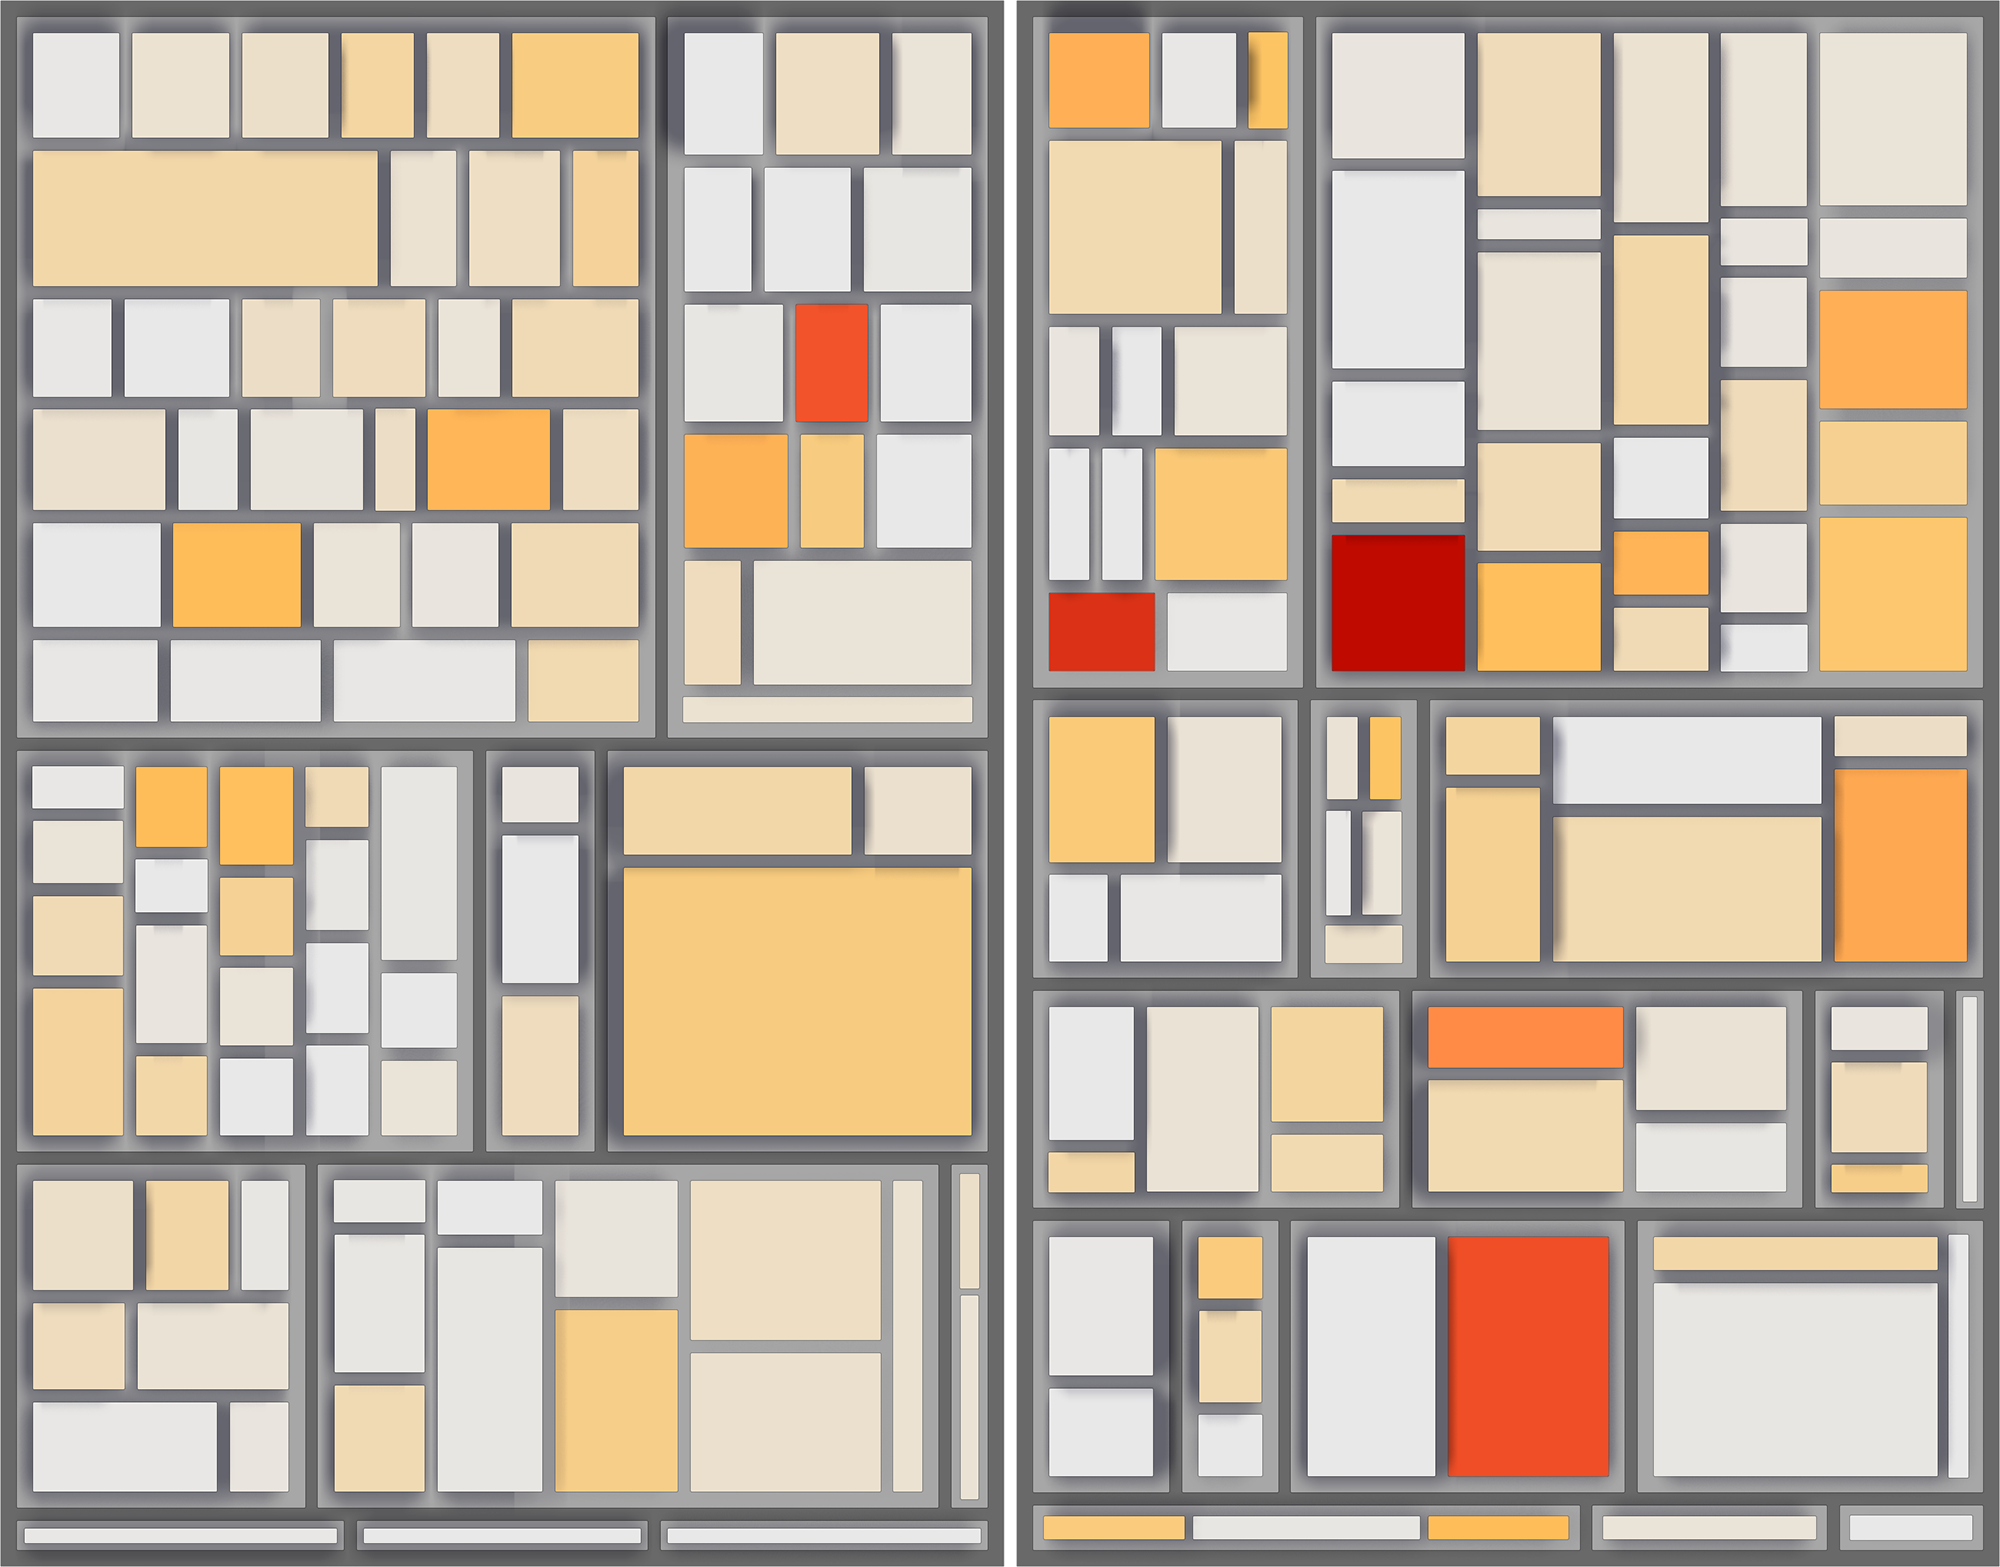
\includegraphics[width=0.9\linewidth]{figures/rectangular-map.png}
			\end{figure}
		\end{column}
	\end{columns}
\end{frame}

\begin{frame}{Future Work}
	\begin{columns}[T,onlytextwidth]
		\begin{column}{0.5\textwidth}
			\textbf{Future Work}
			\begin{itemize}
				\item Refinement of proposed taxonomy
				\begin{itemize}
					\item Evaluation of more tree visualization techniques
					\item Application in tree visualization libraries and software systems
				\end{itemize}
				\item Broadening of the concept of treemaps for tree and hierarchy visualization
			\end{itemize}
		\end{column}
		\begin{column}{0.5\textwidth}
			\centering
			
\includegraphics[width=0.8\linewidth,height=0.8\textheight,keepaspectratio]{images/whitecity_vibrant.png}
		\end{column}
	\end{columns}
\end{frame}
